\chapter{Case Study}
\label{case_study}
\thispagestyle{empty}

In this chapter we focus on our research goal \textbf{RG1.2} as defined in section \ref{research_goals}. In the previous chapter we had worked with synthetic networks and after having conducted several experiments with them with various parameters we wish to now analyze the bias in recommendations for some empirical networks. We start the chapter by talking about the empirical data we wish to use in our thesis and how we process it and set it up for our experiment. We also list down names and few of the network properties for each of the datasets which we use. In the next section we look at the results of our experiment on each of these datasets individually. We primarily analyze the disparate visibility bias for each of the chosen datasets.

\section{Setup}

We work on the \textbf{Facebook100} \cite{traud2012social} dataset published by Traud et. al. in 2011. This huge dataset contains snapshots of Facebook \textit{`friendship networks'} for 100 universities across the United States of America. We choose 4 datasets among the 100 for our thesis and use our recommendation methods on them to receive the recommended nodes list on which we carry out the disparate visibility analysis as we had done previously for \textit{static networks} in section \ref{static_networks}.

\subsection{Dataset overview}

Table \ref{table_facebook_datadet} gives an overview of the networks we choose from the \textbf{Facebook100} dataset to carry out our experiments. The \textbf{NetworkID} is the same as used to identify individual networks in the original dataset. We choose \textit{gender} as the node attribute to distinguish nodes belonging to the \textit{minority} or \textit{majority} group. The \textbf{Minority} column in the table shows the gender representing the minority group in each network. The fraction of nodes which belong to the minority group is given as $f$. We estimate the homophily value for each group using the method outlined by Karimi et. al. \cite{karimi2018homophily}. The minority and majority homophily values are given as $h_{minority}$ and $h_{majority}$ respectively. As we had mentioned earlier in \ref{back_networks}, real-world networks exhibit asymmetric homophily, which we can observe here for the chosen empirical networks. All values for $f$, $h_{minority}$ and $h_{majority}$ have been rounded off to 2 decimal places for our experiments.

\begin{table}[h]
	\centering
	\begin{tabular}{ |c|c|c|c|c|c|c| }
		\hline
		\textbf{Network ID} & \textbf{Total nodes} & \textbf{Total edges} & \textbf{Minority} & \textbf{$f$} & \textbf{$h_{minority}$} & \textbf{$h_{majority}$} \\
		\hline
		Caltech36 & 703 & 15464 & female & 0.32 & 0.75 & 0.6 \\
		Reed98 & 865 & 15948 & male & 0.42 & 0.73 & 0.7 \\
		%Haverford76 & 1350 & 53904 & male & 0.46 & 0.73 & 0.82 \\
		Simmons81 & 1422 & 30486 & male & 0.01 & 0.47 & 0.87 \\
		Swarthmore42 & 1521 & 53726 & male & 0.49 & 0.72 & 0.78 \\
		\hline
	\end{tabular}
	\caption{Details of chosen empirical networks from \textbf{Facebook100} dataset}
	\label{table_facebook_datadet}
\end{table}

We parse the original dataset, which is provided as a sparse matrix to form our own network adjacency matrices. For each network multiple nodes are found to not possess the \textit{gender} information. We choose to discard such nodes and the edges they form from our final network. 

\subsection{Experimental Setup}

For each of the networks $G(V,E)$ chosen by us (as listed in table \ref{table_facebook_datadet}) we use the \textit{Topological} and \textit{Reinforcement} recommender methods (as detailed in chapter \ref{recommender_methods}) to get a recommendation list $L_{v}$ for each node $v \in V$.

Once we have received this recommendation list, we measure the Disparate visibility \cite{fabbri2020effect} for the recommendations (similar to what we did in section \ref{static_networks}). 

\section{Results}

\subsection{Caltech36}

For the network \textbf{Caltech36} \textit{females} form the minority group with 32\% of the nodes belonging to this group. The minority group has a homophily value of 0.75 which is slightly higher than the majority group homophily value of 0.6. 

\begin{SCfigure}[1][h!]
	\centering
	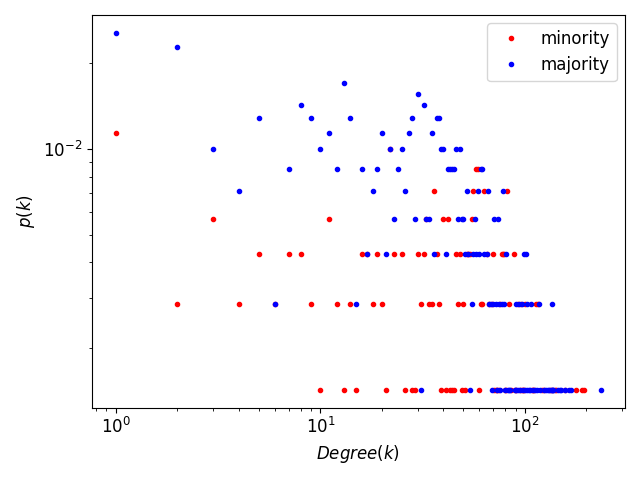
\includegraphics[trim=0 10 0 10, clip, width=0.75\textwidth]{images/dd_caltech.png}
	\caption{Degree distribution for \textbf{Caltech36}}
	\label{dd_caltech}
\end{SCfigure}

Looking at the degree distribution plot (figure \ref{dd_caltech}) we can see that both majority and minority nodes hold quite high degrees. Since both the groups are homophilic in nature with minority being more homophilic, this kind of distribution can be expected for the minority fraction of 0.3. 

\begin{SCfigure}[1][h!]
	\centering
	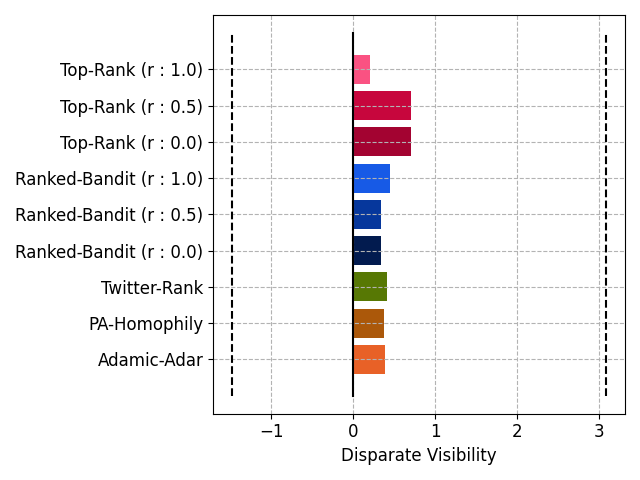
\includegraphics[trim=0 10 0 10, clip, width=0.75\textwidth]{images/dv_caltech.png}
	\caption{Disparate Visibility for \textbf{Caltech36}. Black dotted lines represent the range for the disparate visibility measure given the minority fraction and the solid black line shows the equal visibility mark at 0.}
	\label{dv_caltech}
\end{SCfigure}

Upon using our recommender methods, we find that the disparate visibility (figure \ref{dv_caltech}) is positive, which means that the minority nodes are more visible in recommendations than majorities. This result holds for all recommender methods used. The range of disparate visibility measure for this network lies between [-1.48, 3.08]. 

In our earlier experiments with measuring disparate visibility for static networks in section \ref{static_dv} we had assumed that for a homophilic regime the networks would have higher visibility for majorities. However, here we see that at the homophilic regime minorities are more visible. We however did not have information for the disparate visibility measure at homophily values of $h=0.6$ or $h=0.7$. Thus we might have missed information in our experiments which we can observe in this case. 

For the \textbf{PA-Homophily} method we can deduce that minorities are more visible owing to only slightly high homophily value for majorities and a greater homophily among minorities. This would mean that for both type of nodes there is a higher chance of having minorities as node recommendations. This is also seen in the \textbf{reinforcement methods}. In the case of \textbf{Top-Rank} we see much more visibility for minorities at $r=0.0$ and $r=0.5$, but this visibility decreases from others in the case of $r=1.0$. Here we see that the ranking factor actually has a much more sever effect than what we had observed previously in our experiments with static networks. What we can deduce is that since both minority and majority nodes have higher degrees and they both have only slightly varying homophily, the ranking factor in this case plays a major role in boosting the probability for nodes in \textit{click model}. Lesser visibility for minorities would however mean that the Top-Rank method has a higher mix of majority and minority nodes at upper precedence partitions. This is what causes the minority visibility to drop.

\subsection{Reed98}

For the network \textbf{Reed98}, \textit{males} form the minority group with 42\% of the nodes belonging to this group. The minority group has a homophily value of 0.73 which is very close to the majority group homophily value of 0.7, thus having almost symmetric homophily in this network. 

\begin{SCfigure}[1][h!]
	\centering
	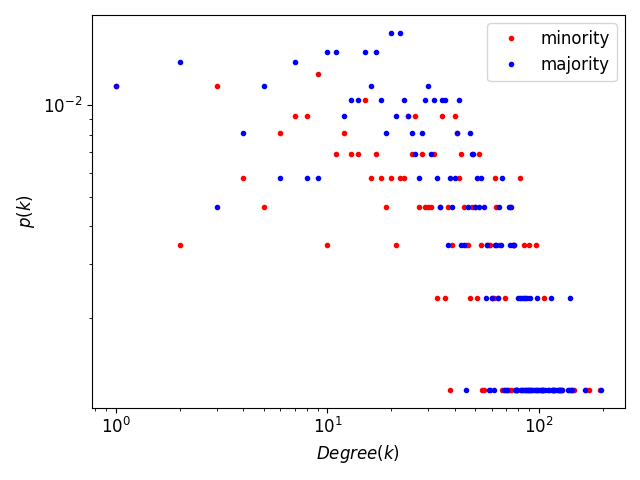
\includegraphics[trim=0 10 0 10, clip, width=0.75\textwidth]{images/dd_reed.png}
	\caption{Degree distribution for \textbf{Reed98}}
	\label{dd_reed}
\end{SCfigure}

Looking at the degree distribution plot (figure \ref{dd_reed}) we can see that both the majority and minority nodes hold high degrees. Since the network is moderately homophilic, with the minority group size quite high this can be expected with both groups supporting themselves. 

\begin{SCfigure}[1][h!]
	\centering
	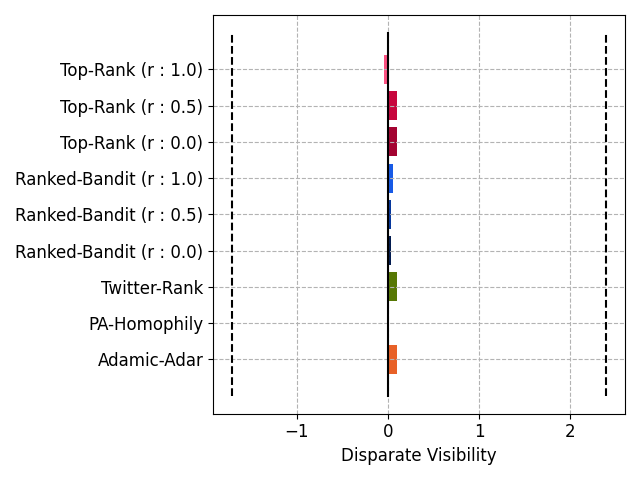
\includegraphics[trim=0 10 0 10, clip, width=0.75\textwidth]{images/dv_reed.png}
	\caption{Disparate Visibility for \textbf{Reed98}. Black dotted lines represent the range for the disparate visibility measure given the minority fraction and the solid black line shows the equal visibility mark at 0.}
	\label{dv_reed}
\end{SCfigure}

From the disparate visibility plot (figure \ref{dv_reed}), upon using our recommender methods on the network, we find that visibility for both groups borders the equal visibility mark. 

We had seen almost equal visibility for a minority size of $f=0.4$ in our synthetic network experiments too. The results corroborate with our findings for this network.

The range for disparate visibility measure for this network lies between [-1.72, 2.4]. Most values are slightly positive which shows that the minority group is at a very slight advantage, but this is very negligible ($\leq 5\%$). The \textbf{Top-Rank} method at $r=1.0$ however shows opposite behavior than the rest, putting majorities as more visible. The behavior which we had seen earlier in the case of \textbf{Caltech36} is thus seen here too for Top-Rank(r=1.0).

\subsection{Simmons81}

For the network \textbf{Simmons81}, \textit{males} form the minority group with only 1\% of the nodes belonging to this group. The minority group has a homophily value of 0.47 while the majority group has a homophily value of 0.87. This is a group with a very less minority who connects in an almost group-agnostic way while the majority has strong homophilic tendencies. So while the majority nodes have strong in-group support they also get connections from the minorities.

\begin{SCfigure}[1][h!]
	\centering
	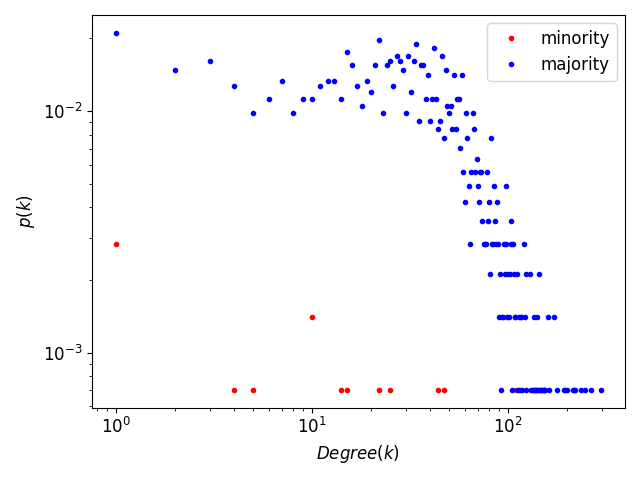
\includegraphics[trim=0 10 0 10, clip, width=0.75\textwidth]{images/dd_simmons.png}
	\caption{Degree distribution for \textbf{Simmons81}}
	\label{dd_simmons}
\end{SCfigure}

Looking at the degree distribution plot (figure \ref{dd_simmons}) we see that the majority nodes hold much higher degrees compared to the minority as we could expect looking at the homophily values. While a fair amount of majority nodes have degrees above 100, the maximum degree a minority node holds is far less than 100. This shows that majority nodes are much more well-connected than minorities.

\begin{SCfigure}[1][h!]
	\centering
	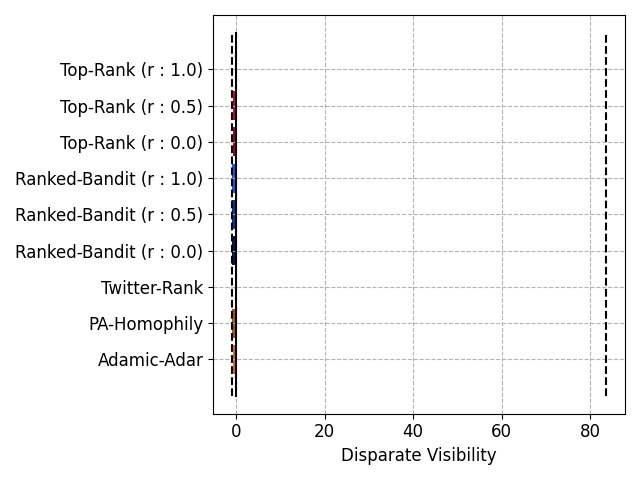
\includegraphics[trim=0 10 0 10, clip, width=0.75\textwidth]{images/dv_simmons.png}
	\caption{Disparate Visibility for \textbf{Simmons81}. Black dotted lines represent the range for the disparate visibility measure given the minority fraction and the solid black line shows the equal visibility mark at 0.}
	\label{dv_simmons}
\end{SCfigure}

From the disparate visibility plot (figure \ref{dv_simmons}), upon using our recommender methods on the nodes in the network, we find that visibility is higher for majority nodes. The range of disparate visibility measure for this network lies in the range of [-1.01, 83.65].

Since the majorities have high homophily and the minorities have almost neutral homophily, the majorities would be winning in the recommendations game in the \textbf{PA-Homophily} and subsequently the \textbf{reinforcement methods} cases. For both the majority and minority nodes there would be more majority nodes which would be suggested. Also since the minorities are so few in number most of them would already be connected with other minorities thus further increasing chances of majorities to be recommended. If the minority group size was higher we would probably see a higher minority visibility for our network. 

\subsection{Swarthmore42}

For the network \textbf{Swarthmore42}, \textit{males} barely form the minority group with 49\% of the nodes belonging to this group. The minority group has a homophily value of 0.72 while the majority group has a homophily value of 0.78. This is a network with equal node-group sizes exhibiting almost symmetric homophilic behavior.

\begin{SCfigure}[1][h!]
	\centering
	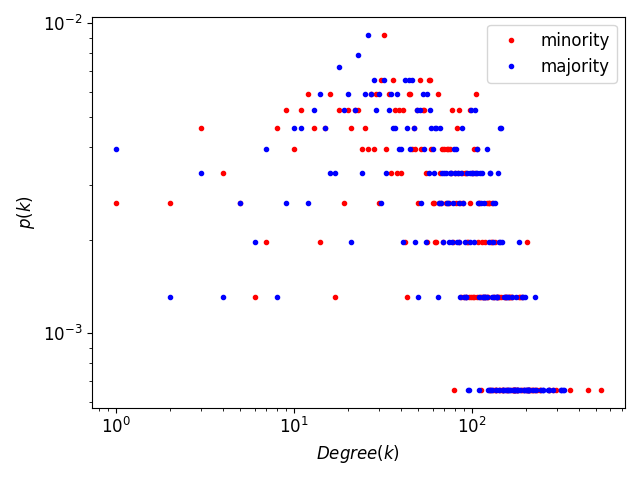
\includegraphics[trim=0 10 0 10, clip, width=0.75\textwidth]{images/dd_swarthmore.png}
	\caption{Degree distribution for \textbf{Swarthmore42}}
	\label{dd_swarthmore}
\end{SCfigure}

Looking at the degree distribution plot (figure \ref{dd_swarthmore}) we see that both majority and minority nodes have an almost equal distribution. The plot however does not strictly demonstrate the properties of a scale-free network as in there are lower degree nodes with lower probability also present in the network. The number of edges in this network is also quite high which would mean that there the nodes are well connected with a higher average degree.

\begin{SCfigure}[1][h!]
	\centering
	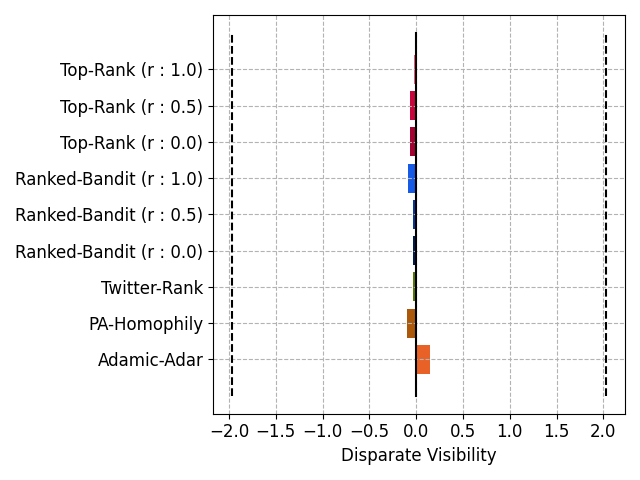
\includegraphics[trim=0 10 0 10, clip, width=0.75\textwidth]{images/dv_swarthmore.png}
	\caption{Disparate Visibility for \textbf{Swarthmore42}. Black dotted lines represent the range for the disparate visibility measure given the minority fraction and the solid black line shows the equal visibility mark at 0.}
	\label{dv_swarthmore}
\end{SCfigure}

From the disparate visibility plot (figure \ref{dv_swarthmore}), upon using our recommender methods on the network, we find that visibility for most cases is only negligibly higher for majority nodes. This suggests that the recommendations are quite balanced for both groups as we could have expected for a equal group size. The range of disparate visibility measure for this network lies between [-1.97, 2.03]. 

For the case of \textbf{Adamic-Adar} we see that the minority seems to have higher visibility than what is projected by the other methods. As we know that the Adamic-Adar method is completely structure dependent this could mean the network structure favors minorities in certain way. However this difference is very negligible to make a concrete comment on why this happens.

\section{Summary}

Using the various recommendation methods $R$ as we had defined in chapter \ref{recommender_methods} we carry out our experiment on empirical networks to get recommendations for each node in the networks. We use selected network from the \textbf{Facebook100} dataset to measure the disparate visibility found in the recommendations.

From our experiments we only see the \textbf{Caltech36} network give a higher visibility score in favor of minorities. The other networks either have an almost equal group-size or have a very small minority size which puts them close to the equal visibility measure.

In \textbf{Caltech36} we see that minorities are more visible which is different from what we were expecting from our experiments on synthetic networks. This clearly points to a limitation of our work since we do not know the disparate visibility behavior in the in-between homophily cases. Our consideration of homophily values for experiments is limited and the behavior in more such cases is something worth exploring in the future.